% =====================
% Chapter 8: Functions (Beginner Friendly, Architecture-Focused)
% Audience: Architecture students new to coding
% Style: uses \h, \hh, \hhh, \code, and NoteBox; code blocks keep your \code indentation
% =====================

\h{Functions}
In architectural design, we often use repeatable, modular components---such as standardized window frames or pre-fabricated wall panels---to streamline the construction process and ensure consistency. In programming, functions serve a similar purpose. They are blocks of organized, reusable code designed to perform a single, specific task. By using functions, we can break down complex problems into smaller, more manageable units, making our programs easier to write, read, and maintain.

\medskip
\textbf{What is a Function?}\\
A function is a named sequence of instructions that you can call upon to execute a task. Instead of writing the same code over and over again, you can define a function once and then use it whenever you need it. This not only saves time but also reduces the chance of errors. Figure \ref{fig:function} illustrates the concept of function.

\medskip
\textbf{Defining a Function}\\
You define a function in Python using the def keyword. The basic syntax is as follows:

\code{c10_syntax}{python}{
    def function_name(parameters):
        # 1) Body: do something
        return result  # 2) optional

    #Outcome: This is syntax only; nothing runs until you call function_name(...).
}{General function definition syntax: use def, parentheses for parameters, and an optional return.}

\begin{figure}[htp!]
    \centering
    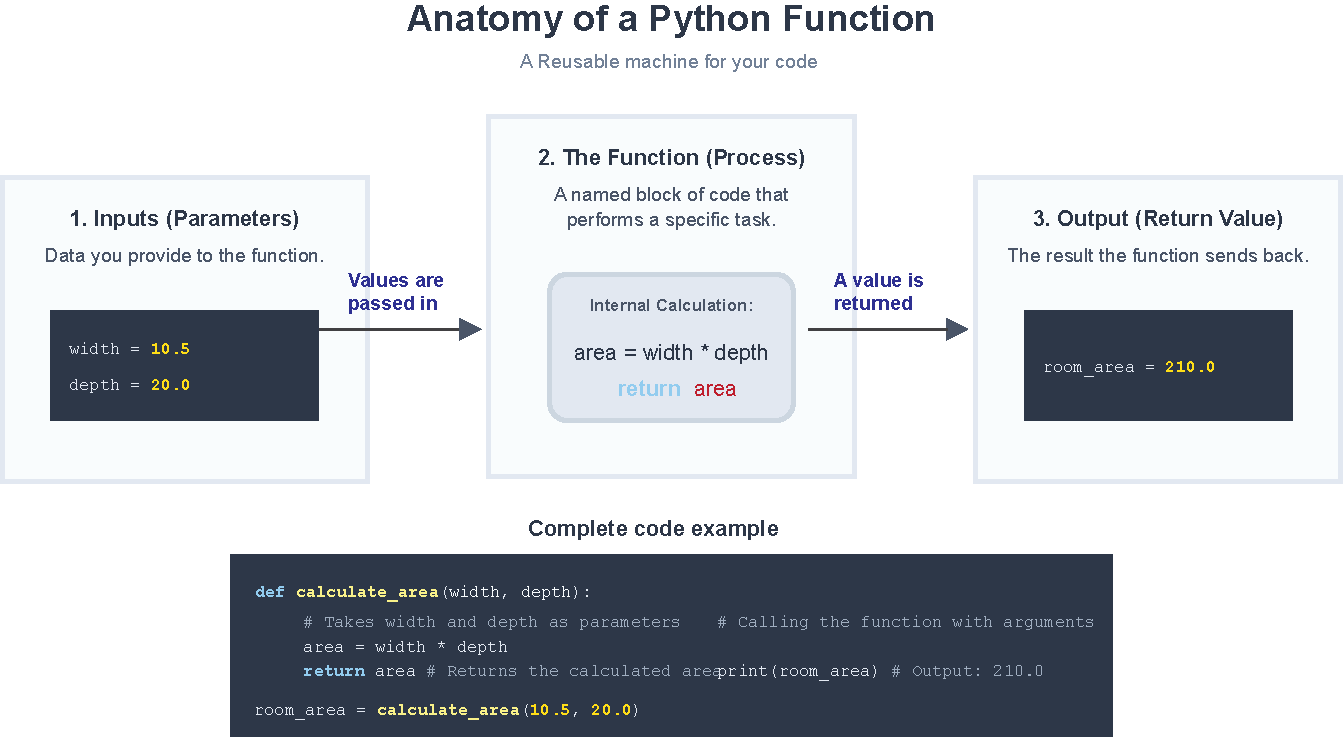
\includegraphics[width=0.75\linewidth]{Figures/Function/Function_Concept.pdf}
    \caption{Anatomy of function}
    \label{fig:function}
\end{figure}

\begin{NoteBox}
\textbf{About this chapter.} A function is a named block of code that runs when called, can accept inputs (parameters), and can optionally return a result. Functions help you organize work, reduce repetition, and make your scripts easier to test and reuse in design workflows. In Python, you define a function with def name(...): and call it by writing name(...).
\end{NoteBox}

\begin{tcolorbox}[% passing options here
    title=Focus of this chapter:,
    colframe=orange,
    colback = white,
%    colback=orange!40!yellow!30, % think of mixing 2 colors with sliders
    arc=2mm % sharp corners
 ]
\begin{itemize}
    \item Defining and calling functions; parameters and return values
    \item Multiple returns (tuples) and unpacking
    \item Defaults and keyword arguments
    \item Docstrings and naming
    \item Scope, pure functions, and side effects
    \item Guard clauses and raising exceptions
    \item Light intro to variable arguments and lambda
    \item Mini-labs to build fluency
\end{itemize}
\end{tcolorbox}

\hh{Conceptual function diagrams}
Let's explore how functions work using simple diagrams. Think of a function as a specialized tool or a small machine in a workshop. We'll visualize how we put raw materials (inputs) into this machine, how it processes them, and what it produces (outputs). Along the way, we'll see how to build bigger workflows by connecting these small machines in a production line (composition), understand the difference between a machine that just gives you a result and one that also changes things elsewhere in the workshop (side effects), and learn how to make our machines safer by checking the raw materials first (guard clauses).

\hhh{A function as a pipeline}
Parameters on the left become inputs; the box computes; the right side is the single return value.

\begin{figure}[h]
\centering
\begin{tikzpicture}[>=Latex, node distance=22mm, line width=0.5pt]
  \tikzset{
    io/.style   ={align=center},
    func/.style ={draw, rounded corners, minimum width=38mm, minimum height=10mm, align=center}
  }
  \node[io]   (in)  { \textbf{Inputs}\\ $w,\;l$ };
  \node[func, right=of in] (f) {\texttt{area\_m2(w,l)}};
  \node[io,   right=of f]  (out) { \textbf{Result}\\ $w\times l$ (m$^2$) };
  \draw[->] (in) -- (f);
  \draw[->] (f) -- (out);
\end{tikzpicture}
\caption{Pipeline: inputs $\rightarrow$ function $\rightarrow$ result (read as \texttt{a = area\_m2(w,l)}).}
\label{fig:c10_func_pipeline_single}
\end{figure}

\hhh{Returning multiple values (tuple)}
One call can return a small bundle; you typically \emph{unpack} it into two names.

\begin{figure}[h]
\centering
\begin{tikzpicture}[>=Latex, node distance=22mm, line width=0.5pt]
  \tikzset{
    io/.style   ={align=center},
    func/.style ={draw, rounded corners, minimum width=44mm, minimum height=12mm, align=center}
  }
  \node[io]   (in)  { \textbf{Inputs}\\ $w,\;l$ };
  \node[func, right=of in] (f) {\texttt{geom(w,l)}\\$\to$ (area, perimeter)};
  \node[io,   right=28mm of f, yshift=6mm] (o1) { \textbf{Result 1}\\ area (m$^2$) };
  \node[io,   right=28mm of f, yshift=-6mm] (o2) { \textbf{Result 2}\\ perimeter (m) };
  \draw[->] (in) -- (f);
  \draw[->] (f) -- (o1);
  \draw[->] (f) -- (o2);
\end{tikzpicture}
\caption{Tuple return: unpack with \texttt{area, per = geom(w,l)} to avoid recomputing.}
\label{fig:c10_func_tuple}
\end{figure}

\hhh{Composition: small steps in a pipeline}
Solve a bigger task by chaining clear, tiny functions—each box is testable alone.

\begin{figure}[h]
\centering
\begin{tikzpicture}[>=Latex, node distance=15mm, line width=0.5pt]
  \tikzset{func/.style={draw, rounded corners, minimum width=38mm, minimum height=10mm, align=center}}
  \node[func] (f1) {\texttt{normalize(label)}};
  \node[func, right=of f1] (f2) {\texttt{area\_m2(w,l)}};
  \node[func, right=of f2] (f3) {\texttt{classify(area)}};
  \draw[->] (f1) -- (f2);
  \draw[->] (f2) -- (f3);
\end{tikzpicture}
\caption{Composition: clean $\rightarrow$ compute $\rightarrow$ decide. Main scripts read like a plan.}
\label{fig:c10_func_pipeline_multi}
\end{figure}

\hhh{Guard clauses (early exits)}
Check for bad inputs first, return early, then keep the “happy path” straight.

\begin{figure}[h]
\centering
\begin{tikzpicture}[>=Latex, node distance=14mm, line width=0.5pt]
  \tikzset{
    block/.style   ={draw, rounded corners, minimum width=44mm, minimum height=8mm, align=center},
    decision/.style={diamond, draw, aspect=2, align=center, inner sep=1.5pt}
  }
  \node[block]    (start)  {\texttt{safe\_density(load, area)}};
  \node[decision, below=of start] (check) {invalid inputs?};
  \node[block,    below left=10mm and 16mm of check] (bad) { \texttt{return None} };
  \node[block,    below right=10mm and 16mm of check] (ok)  { compute \texttt{load/area} };
  \node[block,    below=of ok] (ret) { \texttt{return value} };
  \draw[->] (start) -- (check);
  \draw[->] (check) -- node[left]{Yes} (bad);
  \draw[->] (check) -- node[right]{No} (ok);
  \draw[->] (ok) -- (ret);
\end{tikzpicture}
\caption{Guard first; then compute. Mirrors \texttt{if bad: return None} \textrightarrow{} else compute.}
\label{fig:c10_func_guard_flow}
\end{figure}

\hh{How a Function Runs (Execution Model)}
\begin{itemize}
  \item \textbf{Define:} Python reads \texttt{def name(...):} and stores the function. The body does not run yet.
  \item \textbf{Call:} Writing \texttt{name(...)} executes the body with the given arguments.
  \item \textbf{Return:} \texttt{return value} hands a result back to the caller and stops the function. If no \texttt{return} is given, Python returns \texttt{None}.
\end{itemize}

\code{c10_exec_model}{python}{
    def greet_studio():
        print("Defining the function body...")  # not executed at definition
        return "Hello, ARC Studio!"

    print("1) Before call")
    msg = greet_studio()       # body runs now
    print("2) After call:", msg)

    #Outcome:
    # 1) Before call
    # Defining the function body...
    # 2) After call: Hello, ARC Studio!
}{Definition vs. call: the body executes only when you call the function.}

\hh{Your First Function: Define and Call}
\code{c10_first_fn}{python}{
    def greet_studio():
        """Print a quick greeting for our ARC studio."""
        print("Hello, ARC Studio!")

    # Call (execute) the function
    greet_studio()
    #Outcome: Hello, ARC Studio!
}{Defining a function with def and calling it.}

\hh{Returning a Result}
A function can compute a value and return it to the caller. If you omit return, Python returns None.

\code{c10_room_area}{python}{
    def room_area_m2(width_m: float, length_m: float) -> float:
        """
        Compute rectangular room area in square meters.

        Parameters
        ----------
        width_m : float
        length_m : float

        Returns
        -------
        float : area in m^2
        """
        area = width_m * length_m
        return area

    a1 = room_area_m2(3.5, 5.0)
    print(a1)
    #Outcome: 17.5
}{Returning values with a simple docstring and type hints for readability.}
Modern Python code includes annotations called type hints to make function signatures clearer. Notice the extra labels like \c{: float} and \c{-> float} in the example above. They act as built-in documentation, clarifying what kind of data the function expects as inputs and what it produces as an output.

\hh{Parameters: Positional, Keyword, and Defaults}
You can pass arguments by position or by keyword. You may also set default values for flexibility.

\code{c10_params}{python}{
    def slab_load_kN(area_m2: float, udl_kN_per_m2: float = 3.0) -> float:
        """Uniformly distributed load (kN) on a slab area."""
        return area_m2 * udl_kN_per_m2

    # Positional call:
    q1 = slab_load_kN(120.0, 4.0)
    # Keyword call (order doesn't matter when using keywords):
    q2 = slab_load_kN(udl_kN_per_m2=3.5, area_m2=120.0)
    # Using the default (3.0):
    q3 = slab_load_kN(120.0)

    print(q1, q2, q3)
    #Outcome: 480.0 420.0 360.0
}{Using positional, keyword, and default arguments.}

\hhh{Advanced Parameters: *args and **kwargs (Optional)}
In Python, we use * and ** in function parameters to allow a function to accept a variable number of arguments. This makes functions more flexible.Useful when the exact inputs vary.
\begin{itemize}
    \item *args collects any number of positional arguments into a tuple.
    \item **kwargs collects any number of keyword arguments into a dictionary.
\end{itemize}

\code{c10_args_kwargs}{python}{
    def total_area_m2(*rects, round_to=None, **options):
        """
        Sum areas of any number of rectangular rooms.
        Each rect is a (width_m, length_m) tuple.
        Options (kwargs): can include a 'unit' for  formatted output.
        """
        total = 0.0
        for (w, l) in rects:
            total += w * l
        
        if round_to is not None:
            total = round(total, round_to)
    
        # Check if the 'unit' key exists in the options dictionary
        if 'unit' in options:
            # If it exists, return a formatted string with the unit
            unit_string = options['unit']
            return f"{total} {unit_string}"
        else:
            # Otherwise, return the number as before
            return total

    # This call has no 'unit' option, so it returns a number.
    print(total_area_m2((3.0, 5.0), (4.0, 3.5)))

    # This call includes unit="m2", so it returns a formatted string.
    print(total_area_m2((3.0, 5.0), (4.0, 3.5), round_to=2, unit="m2"))
}{Flexible signatures with *args and **kwargs.}

\hhh{Argument Unpacking When Calling}
You can unpack a list/tuple into positional arguments with *, and a dict into keyword arguments with **.

\code{c10_unpack}{python}{
    def paint_cost(area_m2: float, price_per_m2: float = 1.85) -> float:
        return area_m2 * price_per_m2

    args = (42.0, 2.0)                 # positional pair
    kwargs = {"area_m2": 42.0, "price_per_m2": 2.0}  # keywords

    print(paint_cost(*args))
    print(paint_cost(**kwargs))
    print(paint_cost(42)) # default price_per_m2 = 1.85 is used for this function call
    #Outcome:
    # 84.0
    # 84.0
    # 77.7
}{Unpacking arguments with * and **.}
Note the \c{1.85} is a default argument for the \c{price_per_m2} parameter. This means that if you call the function and only provide a value for \c{area_m2}, the function will automatically use 1.85 for the price. It makes the \c{price_per_m2} parameter optional.
\hh{Multiple Returns (Tuples)}
A function can return multiple values (Python returns a tuple).

\code{c10_area_perim}{python}{
    def rect_geo(width_m: float, length_m: float):
        """Return (area_m2, perimeter_m)."""
        area = width_m * length_m
        perim = 2.0 * (width_m + length_m)
        return area, perim

    a, p = rect_geo(3.0, 7.0)
    print("Area:", a, "Perimeter:", p)
    #Outcome: Area: 21.0 Perimeter: 20.0
}{Returning more than one value for convenience.}

\hh{Scope: Local vs. Global (Prefer Local)}
Variables inside a function are local by default. Prefer returning results instead of modifying global state---this makes code easier to test and reuse.\par
In Python, when a function completes its execution and returns, the local variables defined within that function are indeed removed from memory. This is because local variables are stored on the call stack, and when a function finishes, its corresponding stack frame is popped off, effectively deallocating the memory used by those local variables. However, a global variable is not removed from memory when a function completes. It persists for the entire lifetime of your program.

\code{c10_scope}{python}{
    total_area = 0.0  # avoid mutating this globally inside functions

    def add_room_area(width_m, length_m, running_total):
        """Return an updated running total (no globals)."""
        return running_total + (width_m * length_m)

    total_area = add_room_area(4.0, 5.0, total_area)
    total_area = add_room_area(3.2, 6.0, total_area)
    print(total_area)
    #Outcome: 38.2
}{Favor passing and returning values over using global.}

\hhh{Reading a global (allowed) vs. writing a global (careful)}

\code{c10_read_global}{python}{
    tax_rate = 0.08  # global (module-level)

    def price_with_tax(net: float) -> float:
        # Reading a global is fine (no 'global' keyword needed)
        return net * (1 + tax_rate)

    print(price_with_tax(100.0))
    #Outcome: 108.0
}{Reading a global needs no keyword.}

\code{c10_unboundlocal}{python}{
    count = 0

    def bad_increment():
        # This assignment makes 'count' a local name in this scope.
        # Python sees the assignment first and expects a local 'count',
        # but it's not initialized yet -> UnboundLocalError.
        count += 1

    # bad_increment()  # Uncomment to see: UnboundLocalError: cannot access local variable 'count'
}{Assigning to a name makes it local unless declared {global}.}

\hhh{If you {must} mutate a global: use {global} (with a warning)}

\code{c10_write_global}{python}{
    total_rooms = 0

    def add_room(name: str) -> None:
        global total_rooms  # declares we are writing the module-level name
        print(f"Adding room: {name}")
        total_rooms += 1

    add_room("Studio A")
    add_room("Studio B")
    print(total_rooms)
    #Outcome: 2
}{Writing to a global requires the {global} keyword. Use sparingly.}

\textbf{Warning (best practice):}
Overusing globals creates hidden coupling between functions, makes tests brittle, complicates reasoning about order of calls, and can introduce race conditions in concurrent code. Prefer parameters and return values; if you need shared state, favor objects or closures with controlled mutation.


\hh{Using Functions from Other Files (Modules)}
In a large architectural project, you wouldn't put every detail—structural, electrical, and plumbing—onto a single, massive drawing. Instead, you use separate, organized sheets. Python encourages the same clean approach. You can place related, reusable functions into their own `.py` files, called **modules**. Your main script can then **import** these functions, just like assembling a final project from a set of specialized blueprints.

This practice, called modularity, is key to managing complexity. It lets you create a toolbox of reliable, tested functions that can be shared across many different projects.

\begin{figure}[h]
\centering
\begin{tikzpicture}[>=Latex, node distance=24mm, line width=0.5pt]
 \tikzset{
  file/.style ={draw, minimum width=42mm, minimum height=18mm, align=center, fill=gray!10, rounded corners}
 }
 \node[file] (utils) {\textbf{arc\_utils.py} (Toolbox)\\ \texttt{room\_area\_m2}\\ \texttt{slab\_load\_kN}};
 \node[file, right=of utils] (main) {\textbf{main\_project.py}\\ (Main Assembly Script)};
 \draw[->, line width=1pt, color=orange] (main) -- (utils) node[midway, above, font=\small] {\texttt{import arc\_utils}};
\end{tikzpicture}
\caption{Importing a module: \texttt{main\_project.py} gains access to the functions inside \texttt{arc\_utils.py}.}
\label{fig:c10_func_import}
\end{figure}

Assume we have two files in the same folder: \c{arc_utils.py} (our toolbox) and \c{main_project.py} (our main script).

\code{c10_import_module}{python}{
    # File 1: arc_utils.py (our "toolbox" module)
    # ---------------------------------------------
    def room_area_m2(width_m: float, length_m: float) -> float:
        """Compute rectangular room area in square meters."""
        return width_m * length_m

    def slab_load_kN(area_m2: float, udl_kN_per_m2: float = 3.0) -> float:
        """Uniformly distributed load (kN) on a slab area."""
        return area_m2 * udl_kN_per_m2

    # File 2: main_project.py (our main script)
    # ---------------------------------------------
    import arc_utils  # Import the entire toolbox file

    # To use a function, prefix it with the module name and a dot
    area = arc_utils.room_area_m2(5.0, 4.0)
    load = arc_utils.slab_load_kN(area, 4.5)

    print(f"Area: {area} m2, Load: {load} kN")
    #Outcome: Area: 20.0 m2, Load: 90.0 kN
}{Importing a module and calling functions with the \texttt{module\_name.function\_name} syntax.}

\hhh{Making Modules Testable}
How do you test the functions in \c{arc_utils.py} without the test code running every time you import it? You add a special block: \c{if __name__ == "__main__":}. This code is like a set of test notes on a blueprint. It's ignored when the blueprint is used in a larger assembly (when imported), but it is useful when you are examining that single sheet on its own (when running the file directly).

\code{c10_import_main}{python}{
    # File: arc_utils.py (with a self-contained test block)
    # ----------------------------------------------------
    def room_area_m2(width_m: float, length_m: float) -> float:
        """Compute rectangular room area in square meters."""
        if width_m < 0 or length_m < 0:
            return 0.0
        return width_m * length_m

    # This block only runs when you execute `python arc_utils.py`
    # It does NOT run when imported by another file.
    if __name__ == "__main__":
        print("--- Running tests for arc_utils ---")
        test_area = room_area_m2(10.0, 5.0)
        print(f"Test case (10x5) -> Area: {test_area}")
        assert test_area == 50.0
        
        neg_area = room_area_m2(-5.0, 10.0)
        print(f"Test case (-5x10) -> Area: {neg_area}")
        assert neg_area == 0.0
        print("--- Tests passed! ---")
}{Adding a test block with \texttt{if \_\_name\_\_ == "\_\_main\_\_"} makes your modules reusable and easy to verify.}


\hh{Common Pitfalls for Beginners}
\hhh{Pitfall: Mutable Defaults}
Default argument values are created once, when the function is defined. If you use a mutable object like a list or dictionary as a default, it will be shared across all calls to that function, leading to unexpected behavior. The standard solution is to use `None` as the default and create a new list or dictionary inside the function.

\code{c10_mutable_default}{python}{
    # Bad: shares the same list across all calls
    def add_room_bad(name, rooms=[]):
        rooms.append(name)
        return rooms

    list1 = add_room_bad("Studio A")
    print(list1)
    list2 = add_room_bad("Studio B") # Unexpectedly modifies the same list!
    print(list2)

    # Good: use None and create a new list inside the function
    def add_room_good(name, rooms=None):
        if rooms is None:
            rooms = []
        rooms.append(name)
        return rooms

    list3 = add_room_good("Studio A")
    print(list3)
    list4 = add_room_good("Studio B") # Works as expected
    print(list4)
    #Outcome:
    # ['Studio A']
    # ['Studio A', 'Studio B']
    # ['Studio A']
    # ['Studio B']
}{Avoid mutable defaults: prefer `None` and then create the object inside the function.}


\hhh{Pitfall: Mutable Defaults}
Default argument values are evaluated once (at definition time). Avoid using mutable objects (lists/dicts) as defaults. Use None and create a new object inside instead.

\code{c10_mutable_default}{python}{
    # Bad: shares the same list across calls
    def add_room_bad(name, rooms=[]):
        rooms.append(name)
        return rooms

    print(add_room_bad("Studio A"))
    print(add_room_bad("Studio B"))  # unexpected carry-over!

    # Good: use None and create inside
    def add_room(name, rooms=None):
        if rooms is None:
            rooms = []
        rooms.append(name)
        return rooms

    print(add_room("Studio A"))
    print(add_room("Studio B"))
    #Outcome:
    # Bad prints ['Studio A'] then ['Studio A', 'Studio B']
    # Good prints ['Studio A'] then ['Studio B']
}{Avoid mutable defaults: prefer None then create inside.}

\hhh{Pitfall: Mutating Inputs Inside a Function}
Be careful when modifying a list/dict passed in---changes persist outside. Make a copy if you need to preserve the caller's data.

\code{c10_mutation}{python}{
    def append_room_inplace(rooms, name):
        rooms.append(name)  # mutates the caller's list!
        return rooms

    def append_room_copy(rooms, name):
        new_list = rooms.copy()  # shallow copy
        new_list.append(name)
        return new_list

    orig = ["A"]
    print(append_room_inplace(orig, "B"), "orig:", orig)  # orig changed!
    orig = ["A"]
    print(append_room_copy(orig, "B"), "orig:", orig)     # orig preserved
    #Outcome:
    # ['A', 'B'] orig: ['A', 'B']
    # ['A', 'B'] orig: ['A']
}{Mutating inputs vs. copying to avoid side effects.}

\hh{Writing Clear, Testable Functions}
Key essentials for beginners:
\begin{itemize}
  \item Name functions with verbs and units (room\_area\_m2, slab\_load\_kN).
  \item Keep each function focused on one task.
  \item Prefer short, readable bodies; return early on invalid input.
  \item Document with a brief docstring describing purpose, parameters, and return.
\end{itemize}

\code{c10_validate}{python}{
    def room_area_m2(width_m: float, length_m: float) -> float:
        """
        Compute rectangular room area in square meters.
    
        Parameters
        ----------
        width_m : float
        length_m : float
    
        Returns
        -------
        float : area in m^2
        """
        area = width_m * length_m
        return area
    
    a1 = room_area_m2(3.5, 5.0)
    print(a1)
    #Outcome: 17.5
    # --- End helpers ---


    def carpet_cost(area_m2: float, material: str, price_map: dict) -> float:
        """
        Compute carpet cost given an area and a price table.
        """
        if area_m2 <= 0:
            return 0.0  # early return: nothing to buy
        if material not in price_map:
            raise ValueError(f"Unknown material: {material}")
        return area_m2 * price_map[material]

    materials = {"Carpet": 4.50, "Hardwood": 12.00, "Tile": 9.75}
    a = room_area_m2(3.8, 4.2)
    print(round(carpet_cost(a, "Carpet", materials), 2))
    #Outcome: 71.82
}{Single-responsibility function with early returns and basic validation.}

\hh{Docstrings and help()}
Docstrings (triple-quoted strings immediately inside your function) are shown by help() and many IDEs. Write a one-sentence summary plus short parameter/return notes.

\code{c10_doc_help}{python}{
    def beam_spacing_m(span_m: float, n_spans: int) -> float:
        """Return equal beam spacing (m) across a span."""
        return span_m / (n_spans + 1)

    # Interactive help (works in a Python shell/REPL)
    # help(beam_spacing_m)

    print(beam_spacing_m(12.0, 3))
    #Outcome: 3.0
}{Docstrings appear in interactive help tools (uncomment help(...) in a REPL).}

\hh{Small Helpers: lambda (Optional)}
For tiny, throwaway computations---like a custom sort key---you can use lambda. Keep it short; otherwise prefer a named function.

\code{c10_lambda}{python}{
    rooms = [
        {"name": "A", "w": 3.0, "l": 5.0},
        {"name": "B", "w": 4.0, "l": 3.5},
        {"name": "C", "w": 2.8, "l": 6.0},
    ]

    # Sort rooms by area using a tiny lambda (anonymous function)
    rooms_sorted = sorted(rooms, key=lambda r: r["w"] * r["l"])
    print([r["name"] for r in rooms_sorted])
    #Outcome: ['B', 'A', 'C']  (areas: 14.0, 15.0, 16.8)
}{Use lambda for a brief, inline function.}

\hh{Putting It Together: A Mini Workflow}
\code{c10_workflow}{python}{
    def carpet_cost(area_m2: float, material: str, price_map: dict) -> float:
        """
        Compute carpet cost given an area and a price table.
        """
        if area_m2 <= 0:
            return 0.0  # early return: nothing to buy
        if material not in price_map:
            raise ValueError(f"Unknown material: {material}")
        return area_m2 * price_map[material]
    
    materials = {"Carpet": 4.50, "Hardwood": 12.00, "Tile": 9.75}
    a = room_area_m2(3.8, 4.2)
    print(round(carpet_cost(a, "Carpet", materials), 2))
    #Outcome: 71.82

    def room_area_m2(width_m: float, length_m: float) -> float:
        """
        Compute rectangular room area in square meters.
    
        Parameters
        ----------
        width_m : float
        length_m : float
    
        Returns
        -------
        float : area in m^2
        """
        area = width_m * length_m
        return area
    
    a1 = room_area_m2(3.5, 5.0)
    print(a1)
    #Outcome: 17.5
    # --- End helpers ---


    def floor_summary(rooms, price_map):
        """
        Given a list of rooms (width_m, length_m), return (total_area_m2, total_cost).
        """
        total_area = 0.0
        for (w, l) in rooms:
            total_area += room_area_m2(w, l)
        total_cost = carpet_cost(total_area, "Carpet", price_map)
        return total_area, total_cost

    price_table = {"Carpet": 4.50, "Hardwood": 12.00, "Tile": 9.75}
    rooms_list = [(3.2, 4.1), (5.0, 4.0), (2.8, 3.0)]

    area, cost = floor_summary(rooms_list, price_table)
    print(round(area, 2), round(cost, 2))
    #Outcome: 30.66 138.0
}{Composing small, focused functions into a simple workflow.}

\hh{Exercises}
\begin{enumerate}
  \item Function basics. Write \texttt{triangle\_area\_m2(b, h)} that returns base*height/2. Test it with \texttt{b=6.0}, \texttt{h=3.0}.
  \item Defaults and keywords. Write \texttt{paint\_cost(area\_m2, price\_per\_m2=1.85)} and call it both positionally and with keywords.
  \item Validation. Extend \texttt{carpet\_cost} to accept a \texttt{waste\_factor} (default 0.05). Clamp it between 0 and 0.15 and raise \texttt{ValueError} otherwise.
  \item Multiple returns. Write \texttt{room\_stats(w, l)} that returns area, perimeter, and aspect ratio.
  \item Mini lab. Build \texttt{estimate\_floor(rooms, material, price\_map)} that sums areas, applies a material choice, and returns a formatted string with total area and total cost.
\end{enumerate}

\hh{Key Takeaways}
\begin{tcolorbox}[% passing options here
    colframe=orange,
    colback = white,
%    colback=orange!40!yellow!30, % think of mixing 2 colors with sliders
    arc=2mm % sharp corners
 ]
\begin{itemize}
  \item Functions encapsulate a task, accept inputs, and may return outputs (or None).
  \item Clear names, small scope, and docstrings make your code easier to read and reuse.
  \item Use defaults and keyword arguments for flexibility; avoid mutable default values.
  \item Be mindful of side effects: avoid mutating inputs unless intended; prefer pure functions.
  \item Compose small functions to build workflows for design tasks (areas, loads, costs).
\end{itemize}
\end{tcolorbox}
